\chapter{Méthodes étudiées}
Depuis que Ian Goodfellow a proposé le GAN (Generative Adversarial Network) en 2014, la recherche sur le GAN est très active. Diverses variantes du GAN ne cessent d'apparaître. Yann LeCun a même déclaré que le GAN était \og{}adversarial training is the coolest thing since sliced bread.\fg{} en 2016. Nous nous donc focaliserons dans un sur la génération de paires d'images visuellement similaires via des GANs.

\section{Generative Adversarial Network}

\begin{figure}[H] 
	\centering 
	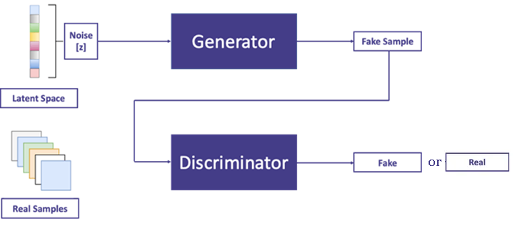
\includegraphics[width=0.6\textwidth]{./resources/img/GAN.png} %插入图片,[]中设置图片大小,{}中是图片文件名
	\caption{architecture GAN} %最终文档中希望显示的图片标题
	\label{Fig3_1} %用于文内引用的标签
\end{figure}

Generative Adversarial Network (GAN) est une méthode d'apprentissage non supervisé, consistant à faire jouer deux réseaux neuronaux l'un contre l'autre. Les GANs se composent d'un réseau génératif (générateur)  et d'un réseau discriminatif (discriminateur). 

\begin{itemize}
	\item \textbf{Le générateur G}, qui apprend à générer des données vraisemblables. Les instances générées deviennent des exemples d'entrainement négatifs pour le discriminateur.
	\item \textbf{Le discriminateur D}, qui apprend à distinguer les fausses données réelles. Il pénalise le générateur lorsqu'il produit des résultats invraisemblables.
\end{itemize}


Dans entraînement de GAN, le générateur génère un échantillon (ex. une image), tandis que son adversaire, le discriminateur essaie de distinguer si cet échantillon est réel ou non. Le but du générateur est de pouvoir tromper le discriminateur autant que possible. Les deux réseaux jouent l'un contre l'autre et ajustent constamment leurs paramètres, dans le but ultime de rendre le discriminateur incapable de déterminer si la sortie du réseau génératif est fausse. 

Au début de l’étape d’entrainement, le générateur produit des données clairement fausses, et le discriminateur apprend rapidement à dire que c’est des fausses données.
Au fur et à mesure que l’entrainement progresse, le générateur se rapproche de la production de données qui peuvent tromper le discriminateur.
Enfin, le discriminateur a de plus en plus du mal à détecter les fausses données. Et commence à les classer comme vraies.


Un des principales contributions de GAN est la stratégie de training qui rend le discriminateur pouvoir reconnaitre la distribution appris par générateur et la distribution réelle. Et, face à des problèmes tels que la difficulté de training, il y a de nombreux améliorations et développements sur l'original tels que c-GAN, cycle-GAN, styleGAN.

\section{pixp2ix} 
pix2pix modèle propose un cadre général pour la tâche de la traduction d'image à image en combinant cGAN pour réaliser la traduction d'image du domaine source au domaine cible. Le réseau apprend non seulement la correspondance entre l'image d'entrée à l'image de sortie, mais apprennent également une fonction de perte pour entraîner cette correspondance. Cela permet d'appliquer la même approche générique à des problèmes qui, traditionnellement nécessiteraient des formulations de perte très différentes\cite{isola2017image}. 

\begin{figure}[H] 
	\centering 
	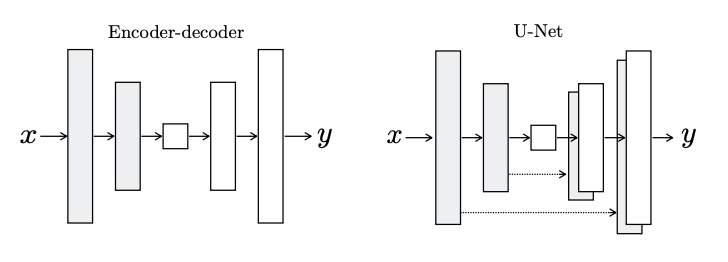
\includegraphics[width=0.6\textwidth]{./resources/img/Unet.jpg} %插入图片,[]中设置图片大小,{}中是图片文件名
	\caption{ U-Net est un encoder-decoder avec skip-connections en forme de miroir entre layers dans l'encoder et dans le decoder} %最终文档中希望显示的图片标题
	\label{Fig3_2} %用于文内引用的标签
\end{figure}

En termes de générateur, pix2pix utilise Unet comme générateur, en considérant que l'aspect de surface des images d'entrée et de sortie doit être différent alors que la structure de base doit être similaire, et que pour la tâche de traduction d'image, l'entrée et la sortie doivent partager certaines informations de base (ex. contours), ils appliquent donc une connexion de layer-skipping comme l'approche de connexion dans Unet.

En termes de discriminateur, l'auteur a crée PatchGAN comme discriminateur, au lieu de  discriminateur qui base sur les distance traditionnelles L1, L2 dans les travaux précédents. L'idée de PatchGAN est de diviser l'image en partie avec over-lapping, ensuite juger la vérité ou la fausseté de chaque patch séparément. Les auteurs concluent en disant que le PatchGAN proposé peut être considéré comme une autre forme de perte de texture ou de perte de style.

Avec pix2pix, si nous fournissons des pairs d'images similaires, nous pouvons former un modèle qui prend une image d'entrée et nous génère une image similaire.


\section{BigGAN et Espace de Latent}

\begin{figure}[H] 
	\centering 
	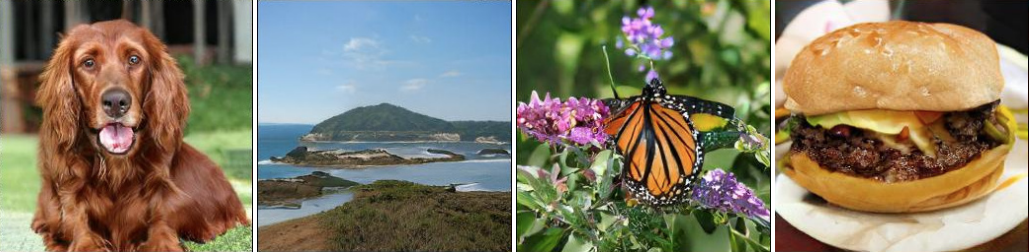
\includegraphics[width=0.6\textwidth]{./resources/img/bigGAN_sample.jpg} %插入图片,[]中设置图片大小,{}中是图片文件名
	\caption{exemples des images généré par BigGAN avec différents vecteur de classe comme entrée\cite{brock2018large}} %最终文档中希望显示的图片标题
	\label{Fig3_2} %用于文内引用的标签
\end{figure}
Grâce à l'avènement des GANs, les algorithmes de modélisation générative d'images ont fait de grands progrès ces dernières années pour générer des images réalistes et diverses. Cependant, la génération d'images diverses et à haute résolution à partir d'ensembles de données complexes comme ImageNet reste une tâche difficile. BigGAN est le modèle génératif le plus grand et le mieux entrainé à ce jour. Les images générées par BigGAN atteignent un niveau de réalisme extrêmement élevé\cite{brock2018large}.

Bien sûr, nous n'avons pas l'intention de former un GAN à partir de zéro, et les modèles de type BigGAN nécessitent d'énormes ressources informatiques pour être formés. Avec l'aide du BigGAN déjà bien formé sur ImageNet, nous considérons essayer de faire varier l'entrée du générateur de manière conditionnelle. Cela implique l'espace latent. \\


\begin{figure}[H] 
	\centering 
	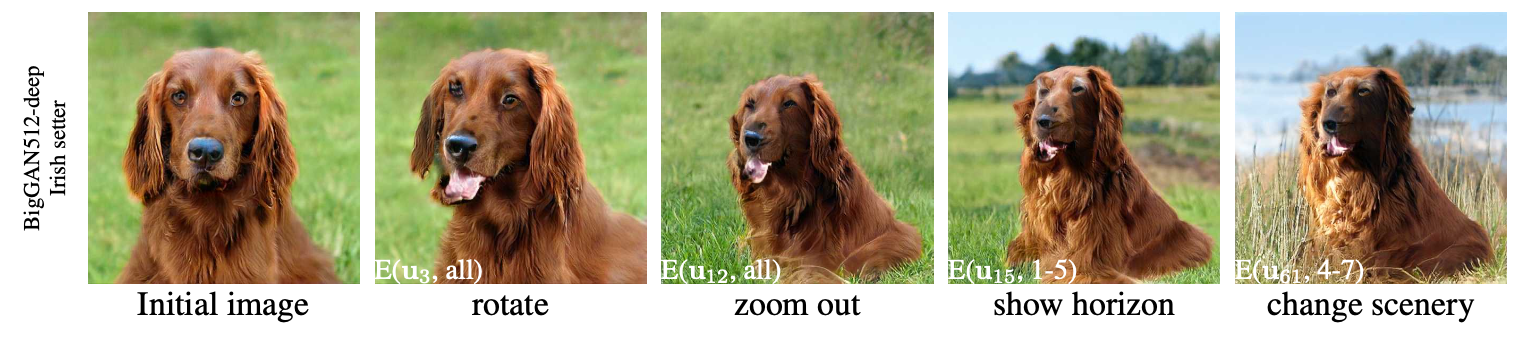
\includegraphics[width=0.6\textwidth]{./resources/img/GANspace.jpg} %插入图片,[]中设置图片大小,{}中是图片文件名
	\caption{exemples des images généré par BigGAN en controlant l'espace latent\cite{harkonen2020ganspace}} %最终文档中希望显示的图片标题
	\label{Fig3_3} %用于文内引用的标签
\end{figure}
Härkönen, Erik, et al\cite{harkonen2020ganspace} décrit une technique simple pour analyser GAN et créer des commandes interprétables pour la synthèse d'images, comme le changement de point de vue, le vieillissement, l'éclairage et l'heure de la journée.

Inspiré par les deux méthodes ci-dessus, nous avons commencé à faire la génération d'image similaire sous condition avec le bien formé BigGAN. 

\begin{figure}[H] 
	\centering 
	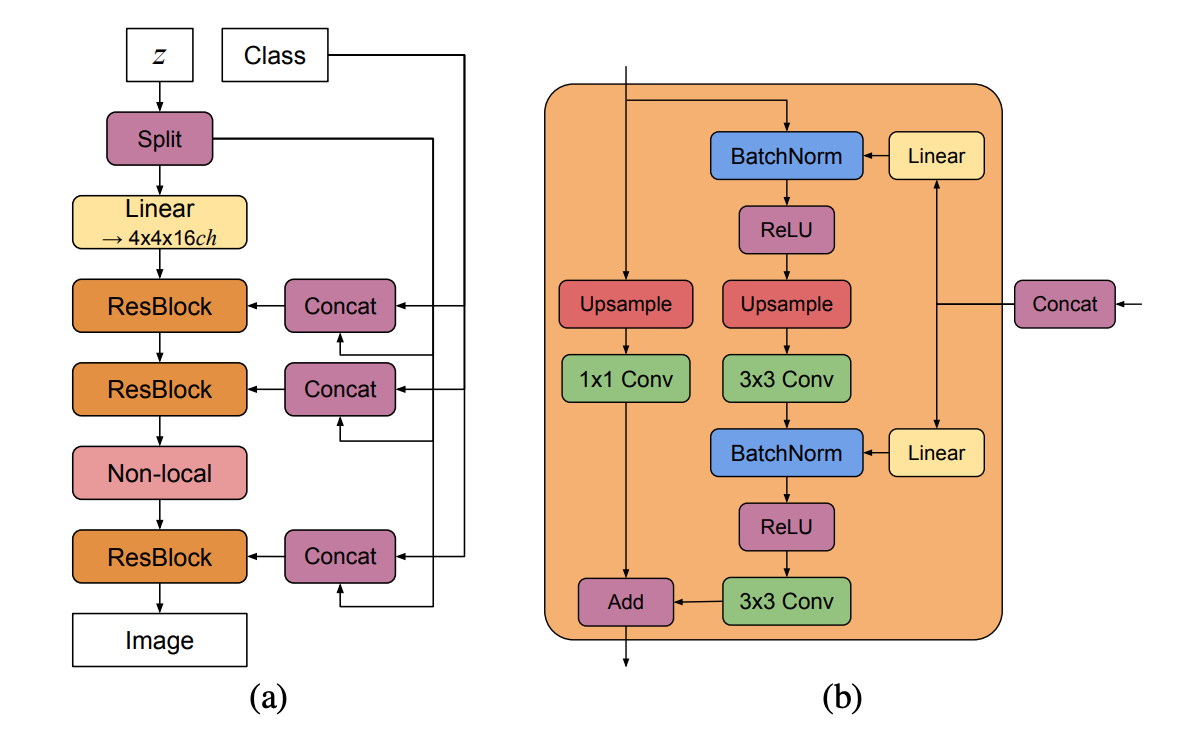
\includegraphics[width=0.8\textwidth]{./resources/img/BigGAN.png} %插入图片,[]中设置图片大小,{}中是图片文件名
	\caption{architecture de BigGAN, (a) est générateur typique, (b) est un  Residual Block de générateur} %最终文档中希望显示的图片标题
	\label{Fig3_4} %用于文内引用的标签
\end{figure}

Si on observe l'architecture, on trouver le générateur prend deux types de vecteur comme latent, le vecteur de bruit (normalement obtenu par la distribution Gaussinne) et le vecteur de classe. En changeant les vecteurs d'entrée, on obtient l'image générée différente. Nous donc déroulons les expériences suivantes, esseyons de définir un loss fonction qui permet d'optimiser la similarité entre l'image généré par BigGAN et l'image donnée. Par exemple construire un singe le plus ressemblant à Einstein qui tire la langue.



